\begin{figure}[tp]
\centering
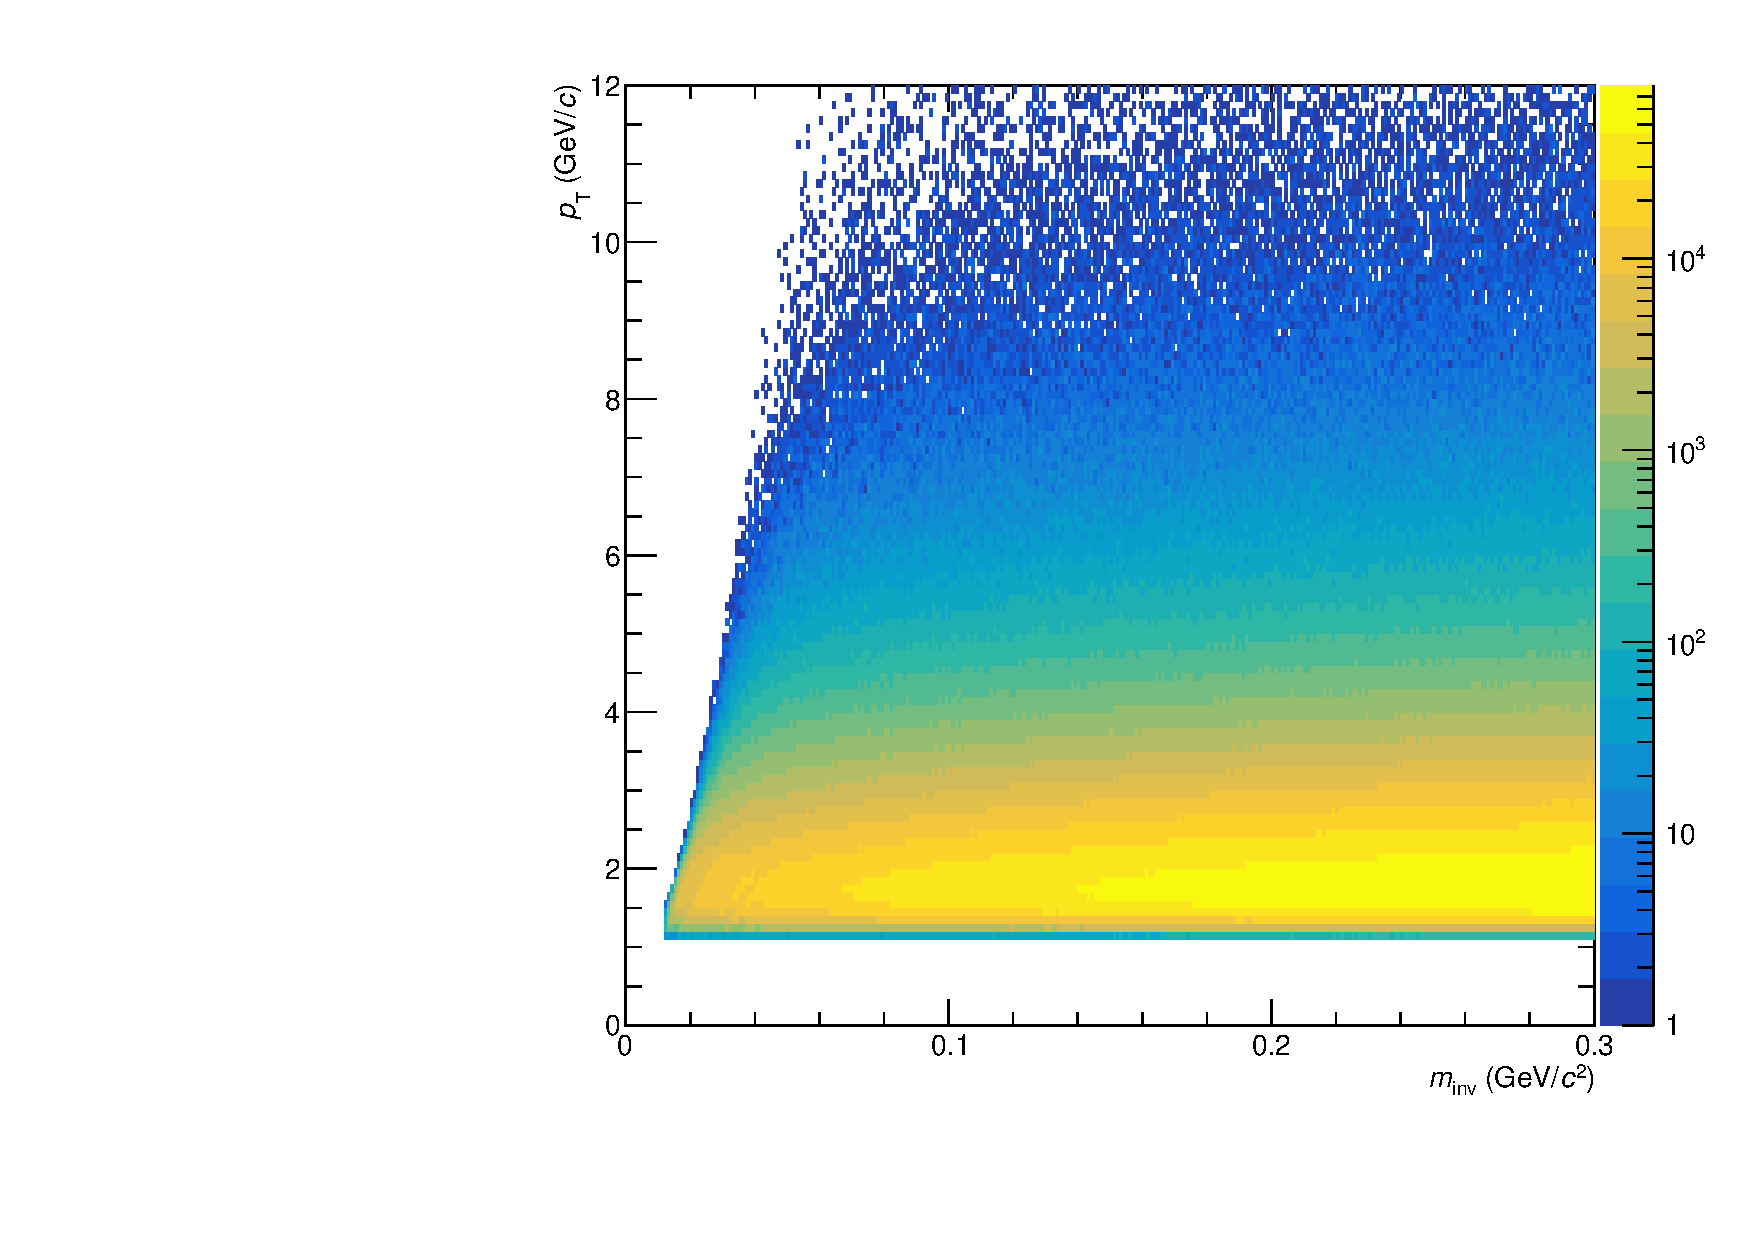
\includegraphics[width=.7\linewidth]{hInvMass_pT_Bkg.pdf}
\caption{$p_\text{T}$ und $m_\text{inv}$ als Funktion von der Anzahl von kombinierten  \tetxit{Clusterpaaren} aus unterschiedlichen \textit{events}.}
\label{figInvMassPt_b}
\end{figure}
Durch das paarweise Kombinieren aller Photonenkandidaten, wie es in Abschnitt \ref{s3s2} vorgestellt wurde, besteht ein großer Anteil der rekonstruierten Datenpunkte aus unkorreliert Paaren.
Um den unkorrelierten Untergrund abzuschätzen werden Photonenkandidaten aus unterschiedlichen \textit{events} paarweise miteinander kombiniert.
Diese Methode wird als \textit{mixed event} Methode bezeichnet.
Abbildung \ref{figInvMassPt_b} zeigt eine Verteilung, bei der Photonenkandidaten aus unterschiedlichen \textit{events} miteinander kombiniert wurden.
Eine Häufung der Datenpunkte um eine bestimmte invariante Masse gibt es, wie zu erwarten, nicht.
Durch die Anforderungen an den Öffnungswinkel sind wieder keine Datenpunkte bei kleinen invarianten Massen zu finden.
Die untere Grenze, ab welcher invarianten Masse Kombinationen möglich sind steigt mit $p_\text{T}$, analog wie zuvor bei Abbildung  \ref{figInvMassPt_a}.
\newline
Aufgrund der größeren Anzahl Einträge, da es in der \textit{mixed event} Methode mehr Kombinationsmöglichkeiten gibt als in der \textit{same event} Methode, muss die Verteilung aus der \textit{mixed event} Methode an die aus der \textit{same event} Methode skaliert werden.
Die Skalierung erfolgt im rechten Bereich außerhalb des $\pi^{0}$-Peaks bei $m_\text{inv} \in \left[0\,19,3\,0\right] (\text{GeV/}c^{2})$ und es ergibt sich für den Skalierungsfaktor:
\begin{align}
\label{eqBackSkalierung}
\alpha &= \frac{\sum_{i \neq j}\sum_{n}m_{\text{inv}}\left( \gamma^{(n)}_{i},\gamma^{(n)}_{j}\right) }{\sum_{i,j}\sum_{n \neq m}m_{\text{inv}}\left( \gamma^{(n)}_{i},\gamma^{(m)}_{j}\right) }
\end{align}
Die oberen Indize $m$ und $n$ stehen hierbei für ein Event, aus dem ein Photon kommt und die unteren Indize $i$ und $j$ numerieren die Photonen ($\gamma$).
\begin{figure}[tp]
\centering
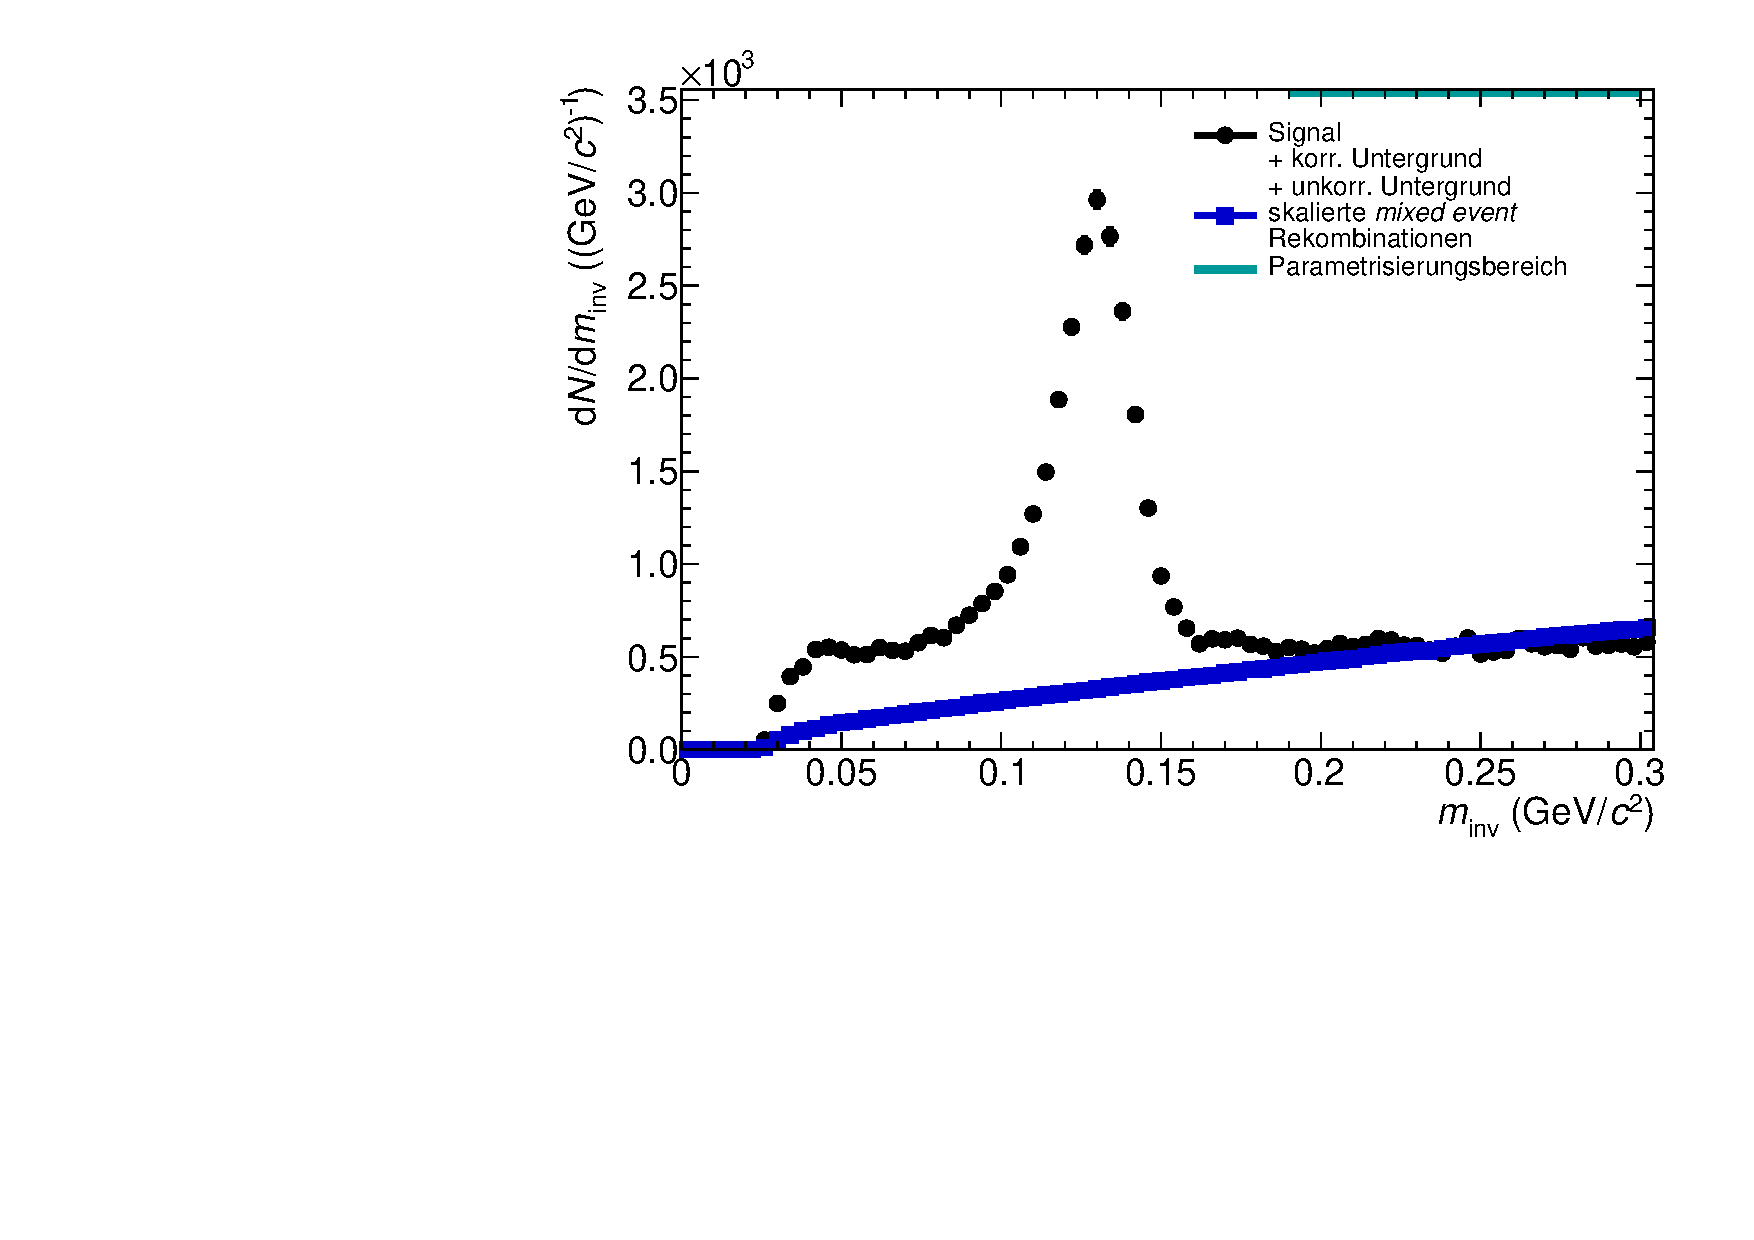
\includegraphics[width=.75\linewidth]{hUncorrBkgNorm.pdf}
\caption{Nach Gleichung \ref{eqBackSkalierung} skalierte {\it mixed event} Kombinationen als Abschätzung des unkorrelierten Untergrunds zusammen aufgetragen mit Signal zuzüglich beiden Untergrundkomponenten wie in Abbildung \ref{figSignalPlusBkg}.}
\label{figUncorrBkgNorm}
\end{figure}
\newline
Das Resultat der Skalierung ist in Abbildung \ref{figUncorrBkgNorm} zu sehen, wo zusätzlich noch das Signal eingezeichnet ist, um besser erkennen zu können, wie sich der abgeschätzte unkorrelierte Untergrund relativ zum gesamten Signal verhält.
Nachdem der unkorrelierte Untergrund abgeschätzt wurde wird dieser vom Signal subtrahiert.
\begin{figure}[tp]
\centering
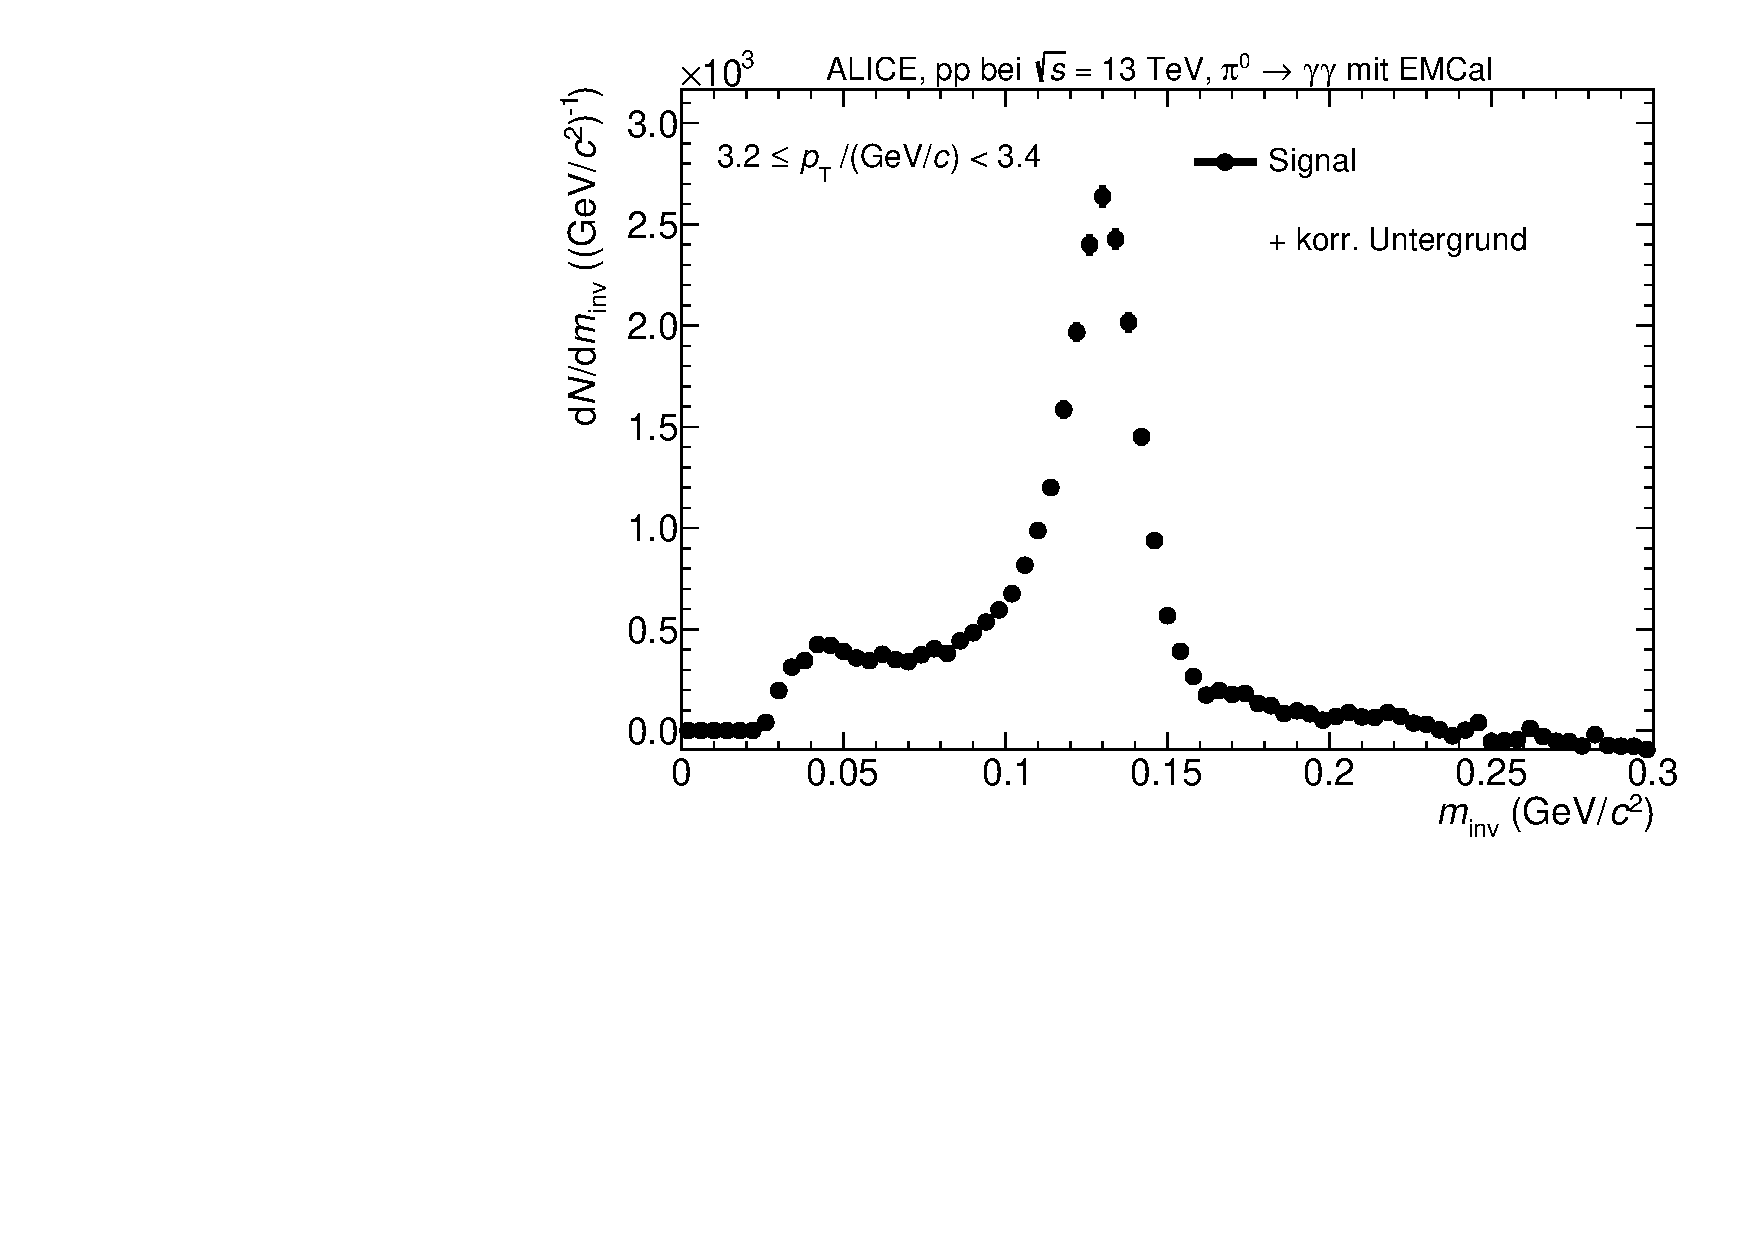
\includegraphics[width=.75\linewidth]{hInvMass_Data.pdf}
\caption{Signal nach Abzug des unkorrelierten Untergrunds.}
\label{figInvMass_Data}
\end{figure}
\newline
Abbildung \ref{figInvMass_Data} zeigt das Ergebnis des Abzugs des unkorrelierten Untergrunds vom Signal.
Da Photonen durch Paarbildung in ein Elektron und ein Positron zerfallen können, bestehen einige Photonenkandidaten aus \textit{Clustern} von nur einem der beiden Zerfallsprodukte.
Diese Photonenkandidaten weisen dann eine geringere Energie auf, als das eigentliche Photon besaß.
Durch Kombinationen mit diesen Photonenkandidaten entstehen Datenpunkte bei einer invarianten Masse, die meistens geringer ist als die Masse von $\pi^{0}$, obwohl beide Photonenkandidaten dem selben $\pi^{0}$ entstammen.
Deshalb wird kleineren invarianten Massen vom Peak ein Teil des Signals erwartet, jedoch auch korrelierter Untergrund.
\newline
Der nächste Schritt in der Analyse neutraler Pionen ist die Bestimmung des korrelierten Untergrunds.
Das Abschätzen mit einer linearen Funktion hat sich zur gängigste Methode zur Bestimmung des korrelierten Untergrunds entwickelt und wird im Folgenden als Standardmethode bezeichnet.
In dieser Arbeit wird der korrelierte Untergrund sowie das reine $\pi^{0}$-Signal mit Hilfe von Templates bestimmt.
Die Ergebnisse der Analyse mit Hilfe von Templates, sowie mit der Standardmethode werden miteinander vergleichen, um eine Aussage über den möglichen Nutzen von Analysen mit Hilfe von Templates treffen zu können.
In den folgenden Abschnitten wird sowohl die Standardmethode kurz, als auch die Methode mit Hilfe von Templates näher erläutert.